\subsection*{Partie A}

\begin{enumerate}
	\item $\mathcal{C}_R$ est une droite passant par l'origine : $R$ est donc une fonction linéaire, de la forme $R(x) = ax$.

	D'après les deux points de coordonnées $(20~;~\np{6000})$ et $(40~;~\np{12000})$ marqués sur le graphique :
	\[a = \dfrac{\np{12000} - \np{6000}}{40 - 20} = \dfrac{\np{6000}}{20} = 300.\]
	
Pour tout $x$ de $[0~;~40]$ : $R(x) = 300x$.

	\item L'entreprise réalise un bénéfice lorsque la recette dépasse le coût, c'est-à-dire lorsque
	$\mathcal{C}_R$ est au-dessus de $\mathcal{C}_C$.

	Par lecture graphique, $\mathcal{C}_R$ est au-dessus de $\mathcal{C}_C$ entre les deux
	points d'intersection des courbes, d'abscisses environ 18 et 39.
	L'entreprise réalise donc un bénéfice pour $x$ compris entre environ
	18 et 39 tonnes.

	\item Le bénéfice est maximal lorsque l'écart vertical
	entre $\mathcal{C}_R$ (au-dessus) et $\mathcal{C}_C$ (en dessous) est le plus grand.

	Avec la précision permise par le graphique, cet écart est maximal pour
	$x \approx 30$ ; le bénéfice maximal est alors d'environ \np{3400}~\euro.
\end{enumerate}

\subsection*{Partie B}

\emph{Pour $x \in [0~;~40]$, $B(x) = -x^3+54x^2-540x-\np{2000}$.}

\begin{enumerate}
	\item Pour tout réel $x$ de $[0~;~40]$ :
	\[B'(x) = -3x^2 + 54 \times 2x - 540 = -3x^2 + 108x - 540.\]
	D'autre part :
	\[(-3x+18)(x-30) = -3x^2 - 90x + 18x - 540 = -3x^2 + 108x - 540.\]
	Donc, pour tout $x$ de $[0 ; 40]$, $B'(x) = (-3x+18)(x-30)$.

	\item $-3x + 18 = 0 \iff x = 6$ (coefficient $-3 < 0$ : positif avant, négatif après) ;

	$x - 30 = 0 \iff x = 30$ (coefficient $1 > 0$ : négatif avant, positif après).

	\begin{center}
		\begin{tikzpicture}
			\tkzTabInit[lgt=3.4,espcl=2.6]
			{$x$/1,$-3x+18$/1,$x-30$/1,$B'(x)$/1,$B$/2}{$0$,$6$,$30$,$40$}
			\tkzTabLine{,+,z,-,,-,}
			\tkzTabLine{,-,,,z,+,}
			\tkzTabLine{,-,z,+,z,-,}
			\tkzTabVar{+/{$-\np{2000}$},-/{$-\np{3512}$},+/{$\np{3400}$},-/{$-\np{1200}$}}
		\end{tikzpicture}
	\end{center}

La fonction $B$ est décroissante sur $[0~;~6]$, croissante sur
	$[6~;~30]$, puis décroissante sur $[30~;~40]$.

	\item D'après le tableau de variations, le bénéfice est maximal pour $x = 30$ tonnes de compote produites et vendues. Il vaut alors $B(30) = \np{3400}$~(\euro).
\end{enumerate}

\medskip
